\begin{refsection}
	\nocite{%Порядок перечисления в этом блоке определяет порядок вывода в списке публикаций автора
		art2,art4,art5,
		art3,art7,
		art8,%art6,
		art1,
		conf5,conf6,conf8,conf9,conf10,%
	}%
	\addtocategory{biblioauthoreng}{art3,art6,art7,art8}
\end{refsection}
\pagenumbering{arabic}

\section*{Загальна характеристика роботи}

\textbf{Актуальність теми дослідження.} 
Системи диспетчерського контролю за рухом автотранспорту призвані ефективно коригувати відхилення від запланованих маршрутів при зіткненні з непередбачуваними обставинами потребують ефективного обміну повідомленнями між водієм і диспетчером. Різні форми автоматизації диспетчерського контролю (GPS, мобільний і супутниковий звязок, сенсорні інтерфейси) на сьогодні не здатні замінити голосову взаємодію, в якій диспетчер отримує необхідну для прийняття рішень інформацію зокрема про характер і причини відхилень від плану. 

Таким чином підвищення ефективності передачі повідомлень за рахунок формалізації голосової взаємодій між водієм та диспетчером є одним із перспективних напрямів вдосконалення системи диспетчерського контролю, що робить тему дисертаційного дослідження інформаційних технологій формалізації голосової інформації в системах диспетчерського контролю за рухом автотранспорту \textbf{актуальною}.

%
%.
%
%.
%
%.
%
%Системи диспетчерського контролю за рухом автотранспорту призвані (у тому числі) ефективно коригувати відхилення від запланованих маршрутів при зіткненні з непередбачуваними обставинами. Інформація про обставини має повідомлятися диспетчеру в найкоротші терміни для забезпечення можливості прийняття ефективних рішень.
%
%В існуючих системах диспетчерського контролю, параметри, такі як GPS трек, повідомляюся диспетчеру у формалізованому вигляді із застосуванням мобільного інтернету або супутникового звʼязку. З цих даних диспетчер має можливість бачити, що характеристика руху не відповідає запланованій, але не має інформації щодо причин такої невідповідності.
%
%Ця інформація може бути отримана за рахунок безпосередньої голосової взаємодії за допомогою мобільного телефону, або у формалізованому вигляді через мобільний додаток водія з сенсорним інтерфейсом.
%
%Водії часто уникають використовувати сенсорний додаток для передачі інформації про причини невідповідності руху та плану, через те що це відволікає від безпосередніх завдань керування автомобілем.
%
%Тобто єдиним каналом отримання цієї інформації залишається безпосередня, неформалізована голосова взаємодія. Проте така голосова взаємодія є витратною по часу як для водіїв так і для диспетчера і використання мобільного телефону є проблемою бо також відволікає від водійських функцій.
% 
%Підвищення ефективності передачі повідомлень є актуальним, оскільки неформалізована голосова взаємодія відбувається часто неефективно, а автоматизована часто уникання.
%
%Все це робить тему дисертаційного дослідження інформаційних технологій формалізації голосової інформації в системах диспетчерського контролю за рухом автотранспорту \textbf{актуальною}.
%
%.
%
%.
%
%.
%
%Системи диспетччерського контрою за рухом автотранспорту призначені для підвищення ефективності своєчасного реагування на незаплановані події.
%
%Вдосконалення систем диспеттчерського контрою призваного коригувати рух автомобіля актуальне в звязку з розвитком автоматизації і ....
%
%.
%
%Системи диспетчерського контролю за рухом автотранспорту призвані ефективно коригувати відхилення від запланованих маршрутів при зіткненні з непередбачуваними обставинами. Інформація про обставини має повідомлятися диспетчеру в найкоротщі терміни і з найменшими витратами часу для ефективних рішень. Голосові повідомлення часто потрибують більше часу і ...
%
%.
%
%.
%
%.
%
%В існуючих системах диспетчерського контролю не використовується голосовий звʼязок «водій --- обладнання автомобіля --- сервер». Всі параметри, такі як GPS трек, передаються диспетчеру у формалізованому вигляді із застосуванням мобільного інтернету або супутникового звʼязку.
%
%Диспетчер бачить що характеристика руху не відповідає запланованій і може її отримати або за рахунок безпосередньої голосової взаємодії за допомогою мобільного телефону, або у формалізованому вигляді через мобільний додаток водія з сенсорним інтерфейсом. 
%
%Водії часто уникають використовувати сенсорний додаток для передачі інформації про причини невідповідності руху та плану, через те що це відволікає від безпосередніх завдань керування автомобілем.
%
%Тобто єдиним каналом отримання цієї інформації залишається безпосередня, неформалізована голосова взаємодія. Проте така голосова взаємодія є витратною по часу як для водіїв так і для диспетчера і використання мобільного телефону є проблемою бо також відволікає від водійських функцій.
%
%.
%
%Формалізація голосової взаємодії потрібна, щоб забезпечити диспетчера швидкою і якісною інформацією про причини збоїв не відволікаючи водія від виконання його основних функцій.
%
%.
%
%
%Під час руху автотранспорту завжди відбуваюся ті чи інші відхилення від плану, які в кожному випадку потребують коригування плану через комунікацію з диспетчером.
%
%.
%
%.
%
%Навіть при отриманні диспетчером всіх параметрі руху у формалізованому вигляді із застосуванням мобільного інтернету або супутникового звʼязку залишається невідомою причина відхилення від плану, що має суттево значення для прийняття диспетчером рішення, щодо подальшого руху автотранспорту.
%
%.
%
%.
%
%.
%
%
%Розвиток прикладних інформаційних технологій на ринку транспортних послуг зумовлений посиленням жорсткої економічної конкуренції та запитом на підвищення екологічності, комфорту та ефективності роботи персоналу.
%
%\ifsynopsis
%\else
%Сьогодні, світові виробники автомобілів, електроніки та телекомунікаційних технологій створюють та використовують компʼютерні інформаційні системи у спроектованих та діючих транспортних засобах. За останні десятиліття, більшість автомобілів набуло оснащення інтерактивними інформаційними системами, що включають аудіо та відео системи, супутникові навігаційні системи, гарнітури телефонії і контроль над кліматом та технічним станом автомобіля. Не дивлячись на те, що такі системи обладнанні дисплеєм, голосова взаємодія з водієм стає все більш широко використовуваною в автомобілях, що допомагає збільшити кількість контрольованих функцій і систем, кнопки яких не можуть бути встановлені на рульовому колесі та приладовій панелі, оскільки обмежено простір. Голосова технологія також дозволяє водіям не відволікатись від управління, знижуючи ймовірність виникнення небезпечних ситуацій на дорозі та підвищуючи безпеку руху. Власними назвами систем голосового управління володіють такі бренди, як Mercedes-Benz, Ford, Cadillac. На марках автомобілів Audi, BMW, Kia, Lexus установлені системи голосового управління для зручності і забезпечення комфорту водіїв. Для систем голосового управління характерна різниця, що полягає у кількості підтримуваних мов, належному рівню при розпізнаванні команд, кількості реалізації функцій управління. Найбільшою кількістю мов володіє система «Ford Sync», крім того арсенал включає і російську мову, але української – немає.
%\fi
%
%У звʼязку з дедалі активнішим використанням природного інтерфейсу і зокрема голосу для спілкування водія з технічними засобами зросло і значення систем голосового управління в самому автомобілі як носія інформації у системах диспетчерського контролю за рухом автотранспорту при здійсненні етапів дистрибуції «склад – дорога – точка доставки».
%
%Не дивлячись на інтенсивний розвиток систем диспетчерського контролю за рухом автотранспорту при взаємодії із водієм, саме голосова інформація потребує формалізації у випадку проведення автоматизації таких систем. Проте існуючі розробки в сфері формалізації голосової інформації поки не пристосовані для аналізу мовлення водіїв, з метою покращення та полегшення їх взаємодії з диспетчерською системою. Саме модель голосової взаємодії водія в системах диспетчерського контролю потребує автоматизації для підвищення ефективності процесу дистрибуції.
%
%Фінальна доставка до дверей клієнта, відома як «остання миля», є одним з найдорожчих та найскладніших у організації дистрибуції. Під час виконання доставки завжди відбуваються ті чи інші відхилення від плану, яким би оптимальним він не був, подібні відхилення в кожному випадку потребують коригування плану через комунікацію з диспетчером. Водії-експедитори та кур'єри скоріше починають виконувати доставки поза планом, якщо процеси комунікації з диспетчером та коригування планів недостатньо прості та ефективні. Для задачі дистрибуції може бути важко забезпечити постійний доступ до мережі інтернет, оскільки доставка може відбуватися до місць/регіонів, де навіть мобільний GPRS інтернет відсутній, або має надто низьку швидкість передачі даних для роботи зі звуком.
%
%Інформаційних технологій які забезпечують автоматизацію голосової взаємодії в системах дистрибуції розроблено не достатньо.
%
%Все це робить тему дисертаційного дослідження інформаційних технологій формалізації голосової інформації в системах диспетчерського контролю за рухом автотранспорту \textbf{актуальною}.

Питаннями автоматизації систем голосового управління займалися такі вчені, як: Бондарос Ю.Г., Волков А.В., Кравченко А.П., Козлов О.С., Корсун О.М., Любімов А.М, Пилипенко В.В., Робейко В.В., Тесля Ю.М., Чорний О.Ю., Чучупал В.Я., Фінаєв І.М., Яцко А.А., Britz D., Deng L., Heisterkamp P., Hinton G., Jonsson I.-M., Kim Y., LeCun Y., Saini P., Yu D., Zhang X., Zhao J.J. та багато інших. Зокрема, результати досліджень голосового управління, заснованих на теорії несилової взаємодії та рефлекторної системи голосового управління належать таким вченим як: Тесля Ю.М., Пилипенко В.В., Чорний О.Ю., Єгорченков А.В.

\textbf{Звʼязок роботи з науковими програмами і планами.}

Дисертаційна робота виконана відповідно до пріоритетного напряму розвитку інформаційних та комунікаційних технологій, що визначені в Законі України «Про пріоритетні напрями розвитку науки і техніки» на період до 2020 року та тематичного плану науково-дослідних робіт Київського національного університету імені Тараса Шевченка в рамках держбюджетної науково-дослідної роботи «Розробка теоретико-методологічних основ впровадження систем управління проектами для розвитку підприємств і організацій» (№ держреєстрації 0117U002694), у якій автор брав участь як виконавець.

\textbf{Обʼєктом дослідження} є процеси голосової взаємодії в системах диспетчерського контролю за рухом автотранспорту.

\textbf{Предмет дослідження} – моделі і методи формалізації голосової взаємодії в системах диспетчерського контролю за рухом автотранспорту.

\textbf{Метою дослідження} підвищення ефективності розпізнавання повідомлень у голосовій взаємодії водія з диспетчером на основі розробки та використання інформаційної технології формалізації голосової інформації в системах диспетчерського контролю за рухом автотранспорту.

Аналіз науково-технічної задачі: розробки моделей і методів формалізації голосової інформації в системах диспетчерського контролю за рухом автотранспорту дозволив сформулювати ряд \textbf{завдань досліджень}, вирішення яких забезпечить досягнення сформульованої мети:

\begin{itemize}
	\item здійснити аналіз сучасних інформаційних систем обробки та формалізації голосової інформації та визначити теоретико-методологічні засади формалізації голосової інформації в системах дистрибуції;
	\item дослідити процес автоматизації руху автотранспорту в дистрибуції та принципи побудови рефлекторної системи голосової взаємодії;
	\item розробити модель та методи формалізації голосової взаємодії в системах диспетчерського контролю за рухом автотранспорту в системі дистрибуції;
	\item провести експериментальні дослідження формалізації голосової інформації, отриманої від водіїв, для оптимізації диспетчерського контролю за рухом автотранспорту при виконанні процесів доставки в системі дистрибуції.
\end{itemize}

\textbf{Методи дослідження}, застосованя для вирішення поставлених завдань: для опису моделі голосової взаємодії — теорія графів, для вдосконалення методу інтелектуальних рефлекторних систем - теорія інформації та теорія несилової взаємодії, для вдосконалення методу згорткових нейронних мереж - теорія штучних нейронних мереж та методи обробки природної мови.

\textbf{Наукова новизна отриманих результатів} полягає в тому, що вперше вирішено наукову проблему інтеграції моделей і методів формалізації голосової інформації з управлінням процесом дистрибуції в єдиній системі формалізації голосової інформації в системах диспетчерського контролю за рухом автотранспорту. При цьому:

\begin{itemize}
	\item вперше створено метод формалізації голосової інформації в допоміжних системах диспетчеризації автотранспорту з використанням інтелектуальних рефлекторних систем, що дозволяє автоматизувати процес голосової комунікації;
	\item удосконалено модель голосової взаємодії субʼєктів дистрибуції в системах диспетчерського контролю за рухом автотранспорту, за рахунок представлення у вигляді повного графу сценаріїв усіх етапів дистрибуції «склад – дорога – точка доставки», що дозволяє виділити контексти голосової взаємодії для підвищення точності подальшої формалізації;
	\item набув подальшого розвитку метод структурної ідентифікації згорткових нейронних мереж для класифікації голосових команд для формалізації голосової інформації в системах диспетчерського контролю за рухом автотранспорту, за рахунок його адаптації для роботи з фонемним текстом, що дозволяє класифікувати голосові команди без переведення голосу в лексичний текст;
	\item отримав подальший розвиток метод інтелектуальних рефлекторних систем для формалізації процесів взаємодії субʼєктів дистрибуції на основі використання теорії нейронних мереж, шо дає можливість оптимізувати значення параметрів шляхом навчання методом зворотного розповсюдження помилки.
\end{itemize}

\textbf{Практичне значення} отриманих результатів полягає в тому, що з використанням наукових результатів, закладається сучасний науково-практичний базис підвищення ефективності управління процесом дистрибуції на основі інформаційної технології формалізації голосової інформації в системах диспетчерського контролю за рухом автотранспорту. Розроблені на базі запропонованих особисто автором моделей і методів програмні засоби становлять практичний результат, який впроваджений на підприємстві ТОВ «Українські Інформаційні Технології».

\textbf{Особистий внесок здобувача.} Наукові положення, розробки та висновки дисертаційної роботи є результатом самостійно проведеного дослідження здобувача. Основні наукові результати, представлені в дисертації, отримані здобувачем особисто.

\textbf{Апробація результатів досліджень.} Основні положення дисертаційної роботи були апробовані на 5-х міжнародних науково-практичних конференціях, в тому числі:

\begin{itemize}
	\item XVII Мiжнародна науково-технiчна конференцiя «Системний аналiз та iнформацiйнi технологiї» (м. Київ, 2015 р.)
	\item XIII Міжнародна конференція «Управління проектами у розвитку суспільства», тема: «Проекти в умовах глобальних загроз, ризиків и викликів» (м. Київ, 2016 р.)
	\item ІІІ Міжнародна науково-практична конференція «Інформаційні технології та взаємодії» (м. Київ, 2016 р.)
	\item 16th EAGE International Conference on Geoinformatics - Theoretical and Applied Aspects (м. Київ, 2017 р.)
	\item ІV Міжнародна науково-практична конференція «Інформаційні технології та взаємодії» (м. Київ, 2017 р.)
\end{itemize}


\printbibliography[heading=countauthor, env=countauthor, keyword=biblioauthor, section=1]%
\printbibliography[heading=countauthorpaper, env=countauthorpaper, keyword=biblioauthor, notkeyword=biblioauthorconf, section=1]%
\printbibliography[heading=countauthorvak, env=countauthorvak, keyword=biblioauthorvak, section=1]%
\printbibliography[heading=countauthorindexed, env=countauthorindexed, keyword=biblioauthorvak, category=biblioauthoreng, section=1]%
\printbibliography[heading=countauthorconf, env=countauthorconf, keyword=biblioauthorconf, section=1]%
\printbibliography[heading=countauthornotvak, env=countauthornotvak, keyword=biblioauthornotvak, section=1]%
\printbibliography[heading=countauthoreng, env=countauthoreng, notkeyword=biblioauthorvak, category=biblioauthoreng, section=1]%

\textbf{Публікації.} 
За результатами дослідження опубліковано 
\formbytotal{citeauthor}{науков}{у працю}{і праці}{их праць} загальним обсягом 9,8 д.а. – 
\formbytotal{citeauthorpaper}{науков}{у статтю}{і статті}{их статей} (3,7 д. а.), у тому числі 
\formbytotal{citeauthorvak}{}{}{}{} у фахових виданнях (з них 
\formbytotal{citeauthorindexed}{стат}{тю}{ті}{ей} у виданнях, які входять до наукометричних баз даних) і 
\formbytotal{citeauthoreng}{}{}{}{} – в іноземному науковому виданні, та 
\formbytotal{citeauthorconf}{роб}{ота}{оти}{іт} в матеріалах і тезах доповідей на наукових конференціях.


 % Характеристика работы по структуре во введении и в автореферате не отличается (ГОСТ Р 7.0.11, пункты 5.3.1 и 9.2.1), потому её загружаем из одного и того же внешнего файла, предварительно задав форму выделения некоторым параметрам

%Диссертационная работа была выполнена при поддержке грантов ...

%\underline{\textbf{Объем и структура работы.}} Диссертация состоит из~введения,
%четырех глав, заключения и~приложения. Полный объем диссертации
%\textbf{ХХХ}~страниц текста с~\textbf{ХХ}~рисунками и~5~таблицами. Список
%литературы содержит \textbf{ХХX}~наименование.

\section*{Основній зміст роботи}
У \textbf{вступі} наведено загальну характеристику роботи, яка підкреслює її
актуальність, відповідність науковим темам, наукову новизну та практичне
значення, визначено предмет та обʼєкт дослідження, сформульовано мету та задачі
дослідження.

У \textbf{першому розділі} «Проблема формалізації голосової інформації в системах диспетчерського контролю за рухом автотранспорту» проведено аналіз сучасних інформаційних систем формалізації голосової інформації, уточнено проблему, гіпотеду та завдання дослідження. 

Розглянувши проблему формалізації голосової інформації в системах диспетчерського контролю за рухом автотранспорту встановлено, що інформаційні технології в управлінні дистрибуцією є достатньо розробленими для забезпечення етапів отримання продукції та її збереження, але недостатньо --- для етапу доставки продукції до кінцевих клієнтів, особливо щодо проблеми «останньої милі». Значну роль в управлінні дистрибуцією відіграють процеси голосової взаємодії, автоматизація яких здатна підвищити ефективність системи дистрибуції.

На сучасному етапі автоматизації голосового управління в організаційно-технічних системах існує проблема своєчасного коригування в необхідних випадках планових маршрутів руху автотранспорту, що інколи призводить до достатньо великих витрат часу на комунікацію, і відповідно є найбільш обґрунтованим напрямом автоматизації голосової взаємодії.

Автоматизація голосової взаємодії для своєчасного коригування планових маршрутів руху автотранспорту повинна доповнити наявні засоби автоматизації управління в системах дистрибуції, такі як відстеження руху автомобілів у режимі реального часу за допомогою GPS треку. Існуючі в дистрибуції системи автоматизації голосової взаємодії для управління зберіганням є занадто спрощеними для використання в задачах доставки.

Проведений аналіз сучасних інформаційних систем формалізації голосової інформації показав, що традиційно вони включають три етапи: попередня обробка з виділенням ознак, перетворення голосової інформації в текстову та виділення змісту з текстової інформації. Такий підхід не в змозі повністю забезпечити автоматизацію голосової взаємодії в задачах управління дистрибуцією, оскільки переведення голосової інформації в лексичний текст потребує встановлення у кабіні водія потужного обладнання або забезпечення стабільного та швидкісного доступу до Інтернету. Висунуто ідею, що розроблення моделі голосової взаємодії без блоку переведення звуку голосу в текст може принципово покращити автоматизацію голосової взаємодії в системах контролю дистрибуції.

Встановлено пріоритетність підходу до голосового управління, заснованого на теорії несилової взаємодії з рефлекторною системою голосового управління. Підхід включає безпосередній аналіз інформаційної складової, вимовленої субʼєктом, з визначенням керуючого впливу з поміж відомих реакцій в певному предметному полі.

В результаті проведеного аналізу сформована основна ідея, гіпотеза, мета та спрямування дослідження, поставлено задачі досліджень дисертаційної роботи. Визначена необхідність в розробці моделей і методів, що дадуть змогу формалізувати голосову інформацію в системах диспетчерського контролю за рухом автотранспорту, тим самим забезпечити підвищення ефективності управління системою дистрибуції.

У \textbf{другому розділі} «Науково-методологічні основи автоматизації голосової взаємодії в системі диспетчеризації» визначено науково-методологічні основи автоматизації голосової взаємодії в системі диспетчеризації. 

Запропоновано концепцію створення системи автоматизації голосової взаємодії в задачах управління дистрибуцією, що має дві складові: (а) інтелектуальні рефлекторні системи голосового управління, що включають блок розпізнавання звукового сигналу та блок виділення його змісту; (б) модель сценаріїв взаємодії у процесах дистрибуції на трьох етапах доставки (завантаження на складі, дорога до точки доставки, розвантаження у точці доставки).

Найбільш перспективним напрямом, який дає змогу запропонувати нове принципове рішення і побудувати рефлекторну модель голосової взаємодії в задачах управління дистрибуцією є застосування моделей логічних сценаріїв взаємодії у процесах дистрибуції, які мають враховувати параметри основних причин невідповідності реальної ситуації запланованому маршруту. При отриманні такої інформації приймається своєчасне рішення про повернення вантажу на склад, про відміну чи відкладення обслуговування однієї точки доставки, щоб мати можливість встигнути на іншу, більш важливу, про зміну маршруту для обʼїзду затору або про утворення нового маршруту з резервною машиною тощо.

Структурування моделі за трьома етапами дистрибуції дає змогу вирішувати проблемні моменти із залученням диспетчера для вибору найкращої стратегії і мінімізації втрат. Структурна модель є принциповим алгоритмом побудови дерева сценаріїв голосової взаємодії для кожного з субʼєктів (диспетчера та водія).

Розроблена система автоматичного розрахунку планових маршрутів та практика її використання забезпечили накопичення параметрів непередбачуваних ситуацій на плановому маршруті доставки, що впливають на створення сценаріїв голосової взаємодії.

Дослідивши методи автоматизації руху автотранспорту в дистрибуції та параметри, що впливають на сценарії голосової взаємодії, розроблено евристичний алгоритм, який максимально враховує вимоги логістів та водіїв щодо оптимальності наповнення кожного конкретного маршруту, забезпечуючи глобальну оптимальність сукупності усіх маршрутів при високій швидкості обчислення.

Завдяки автоматизації голосової взаємодії дані GPS будуть доповнюватися додатковою інформацією про закінчення виконання однієї з точок в межах єдиної зупинки і початок виконання наступної точки. Для забезпечення зазначеного необхідно впровадити зручний інтерфейс, який не буде відволікати водія від основного завдання, тобто голосовий інтерфейс, який сприйматиме команди про початок та завершення виконання доставки.

Модель голосової взаємодії запропоновано будувати у вигляді орієнтованого графу, в якому вершини позначають стан системи та діалогові фрази, які буде озвучувати система, а ребра – репліки (стимули), які можуть бути сприйняті системою в кожній конкретній вершині, а множина всіх ребер, що виходять з однієї вершини, буде позначати перелік стимулів розпізнання для її стану. У результаті для повноцінного опису запропоновано використовувати такі сутності: «контекст» (або «стан»), «стимул» (або «подія») та «реакція» системи відповідно до стимулу.

Принципи побудови рефлекторних систем на основі теорії несилової взаємодії адаптовано для автоматизації голосової взаємодії в системах диспетчерського контролю за рухом автотранспорту.

Під час дослідження принципів побудови рефлекторної системи голосової взаємодії встановлено особливості застосування теорії несилової взаємодії як основи інтелектуальних рефлекторних систем, а також теоретично запропоновано використання рефлекторного методу для побудови рефлекторної системи голосової взаємодії в системах диспетчерського контролю за рухом автотранспорту.


\textbf{Третій розділ} «Методи формалізації голосової інформації в системах диспетчерського контролю за рухом автотранспорту» присвячено створенню моделі та методів формалізації голосової інформації в системах диспетчерського контролю за рухом автотранспорту.

Запропонована класифікація реакцій для субʼєктів дистрибуції на етапах «склад – дорога – точка доставки» базується на узагальненні зібраних статистичних даних щодо процесу доставки різних вантажів автомобільним транспортом у провідних логістичних компаніях України.

Розроблено модель голосової взаємодії субʼєктів дистрибуції в системах диспетчерського контролю за рухом автотранспорту, яка представлена у вигляді повного графу сценаріїв усіх етапів дистрибуції (рис. \ref{img:13_complete_scenario_graph}). 

\begin{figure}[!h]
	\centering
	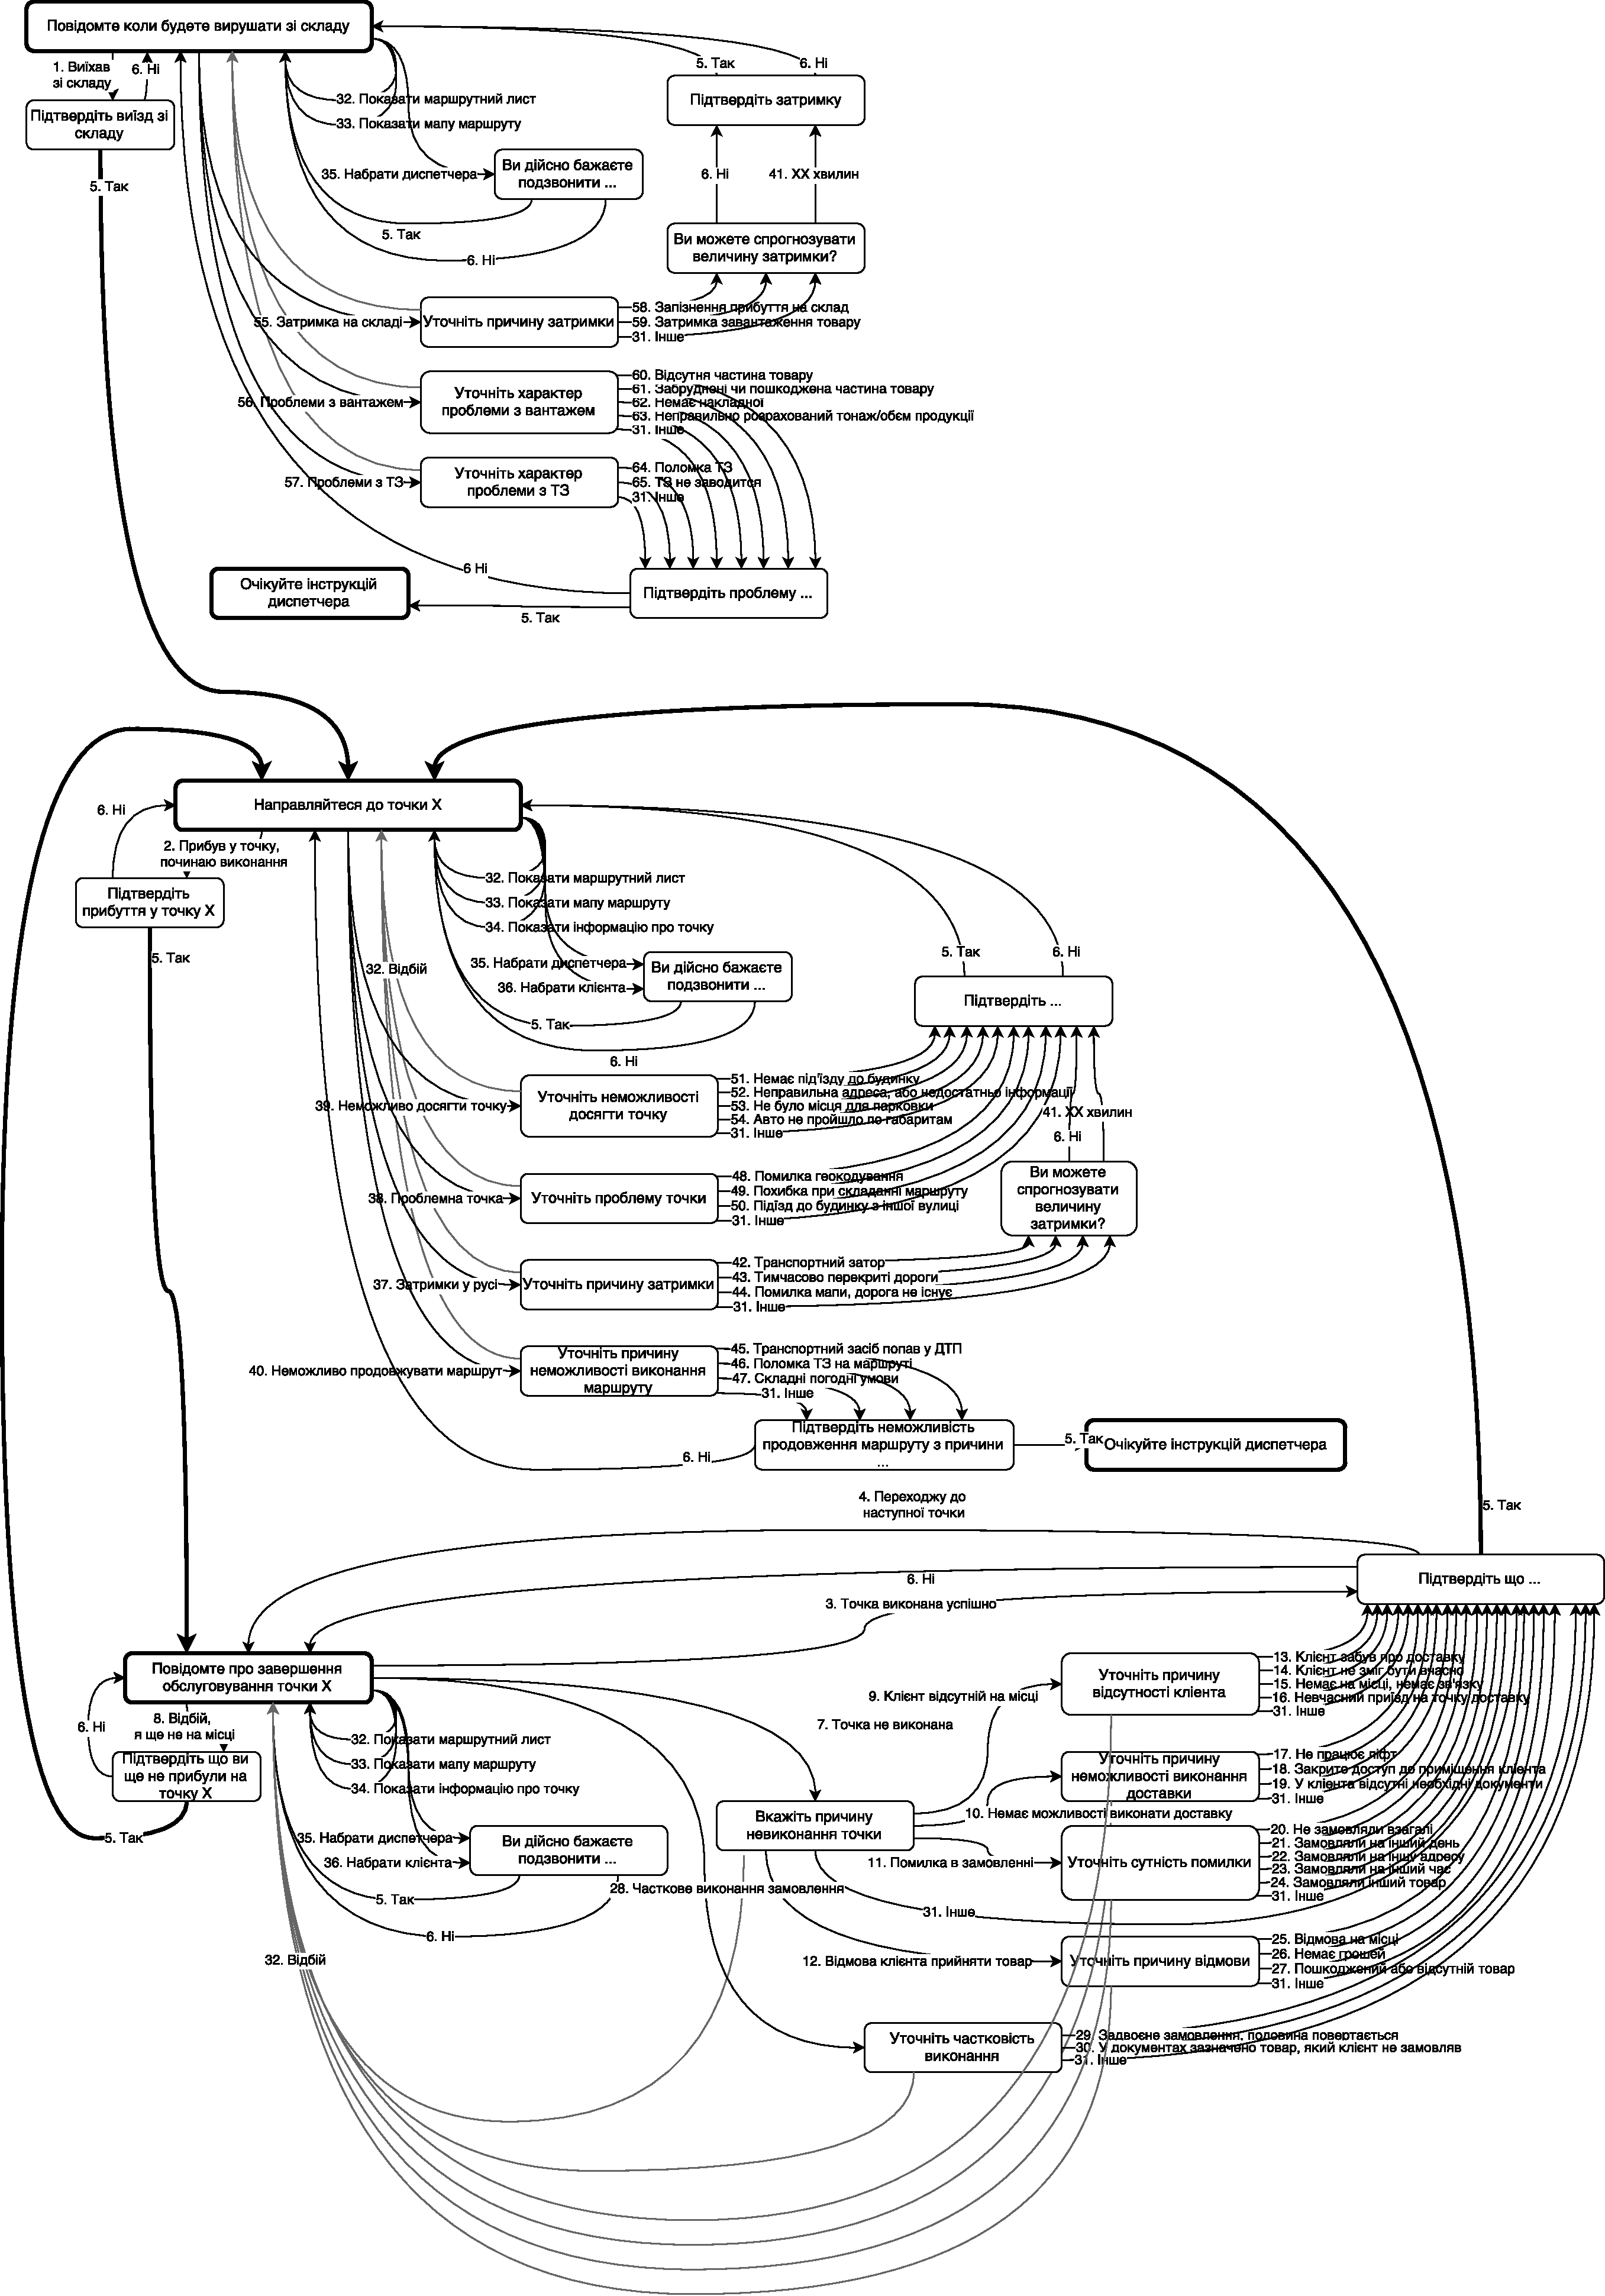
\includegraphics [width=1\linewidth] {13_complete_scenario_graph}
	\caption{Повний граф сценаріїв голосової взаємодії}
	\label{img:13_complete_scenario_graph}
\end{figure}

Для створення контекстної моделі голосової взаємодії в системах диспетчерського контролю за рухом автотранспорту було зібрано статистичні дані, зауваження та коментарі щодо процесу доставки різних вантажів автомобільним транспортом у провідних логістичних компаніях. Систематизувавши та обробивши зібрані оригінальні коментарі до статусу доставки, що використовуються в різних компаніях, розроблено граф сценаріїв взаємодії субʼєктів дистрибуції.

У повному дереві сценаріїв усіх етапів дистрибуції (рис. \ref{img:13_complete_scenario_graph}) враховано всі виявлені можливі причини затримки або невиконання етапів «склад», «дорога», «точка доставки», а для таких випадків існують вказівки (інструкції) диспетчера щодо подальших дій водія.

Модель голосової взаємодії субʼєктів дистрибуції може бути представлена у вигляді орієнтовного графу $G$, що складається з множини вершин $V$ та множини ребер $E$:

\begin{align}
G&=\langle V,E\rangle; \nonumber\\
E&=\{\langle v_i,v_j\rangle | v \in V\}. \nonumber
\end{align}

При цьому існує відношення $f_R$ множини ребер на множину реакцій та відношення $f_C$ множини вершин на множину контекстів, такі що:

\begin{align}
f_R&: E \rightarrow R,\quad R\subset\mathbb{N},\quad |R|\le|E|; \nonumber\\
f_C&: V \rightarrow C,\quad C\subset\mathbb{N},\quad|C|\le|V|; \nonumber\\
R_V(v_i) &= \{f_R(e)|\forall j:e=\langle v_i,v_j\rangle \in E\}; \nonumber\\
\forall i,j: f_C(v_i)&=f_C(v_j) \iff R_V(v_i) = R_V(v_j), \nonumber
\end{align}

\noindent
де $R_V(v_i)$ множина реакцій можливих у вершині $v_i$.

Виділено перелік унікальних контекстів голосової взаємодії, формалізація голосової інформації в яких може відбуватися незалежно один від одного, що дозволяє знизити кількість реакцій для розпізнання.

Адекватність розробленої моделі підтверджується за рахунок того, що вона повністю відповідає статистичним даним інцидентів зібраних за період впровадження системи та експериментально, за рахунок порівняння результатів моделювання з використанням моделі, та без неї.

Метод формалізації голосової інформації в системах підтримки диспетчеризації автотранспорту з використанням інтелектуальних рефлекторних систем дозволяє автоматизувати голосову взаємодію субʼєктів дистрибуції з уникненням переводу звукової інформації в лексичний текст за рахунок використання двох основних модулів (автоматичного фонетичного стенографа і ядра рефлекторної системи голосового управління).

Розроблений метод інтелектуальних рефлекторних систем для формалізації голосової інформації в системах диспетчерського контролю за рухом автотранспорту можна представити наступною послідовністю операцій:

\begin{enumerate}
	\item запис фрази вимовленої водієм: $A_i=\langle a_1,a_2,...,a_n\rangle; t=\frac{n}{s}; s=16 \text{ (kHz)};$
	\item перетворення записаної фрази на фонетичний текст, за допомогою фонемного стенографа: $P_i=S(A_i); P=\langle p_1,p_2,...,p_k\rangle; p_i \in F;$
	\item класифікація фонемної репрезентації голосової команди: $y_i=C_c(P_i);$
	\begin{enumerate}
		\item розбиття фонетичного тексту на N-грами фонем різної довжини;
		\item розрахунок інтроформаційного впливу кожного N-граму фонем на можливі команди в вибраному контексті;
		\item вибір команди з найбільшою ймовірністю;
	\end{enumerate}
	\item виконання відповідної реакції (озвучення відповіді, виконання команди та/або відправка структурованих даних диспетчеру);
	\item переключення контексту на новий, відповідний до вибраної реакції: $c_{i+1} = f(c_i, y_i);$
	\item очікування та запис наступної фрази.
\end{enumerate}


Де: $A_i$ --- цифровий аудіозапис команди водія довжиною $t$ секунд,

{\settowidth{\leftskip}{Де:\ }
	
	$n$ --- кількість семплів аудіо сигналу,
	
	$s$ --- частота дискретизації аудіо сигналу,
	
	$P_i$ --- представлення команди водія у вигляді фонемного тексту --- кортежу фонем довжини $k$,
	
	$F$ --- множина фонем української мови,
	
	$S$ --- фонемний стенограф,
	
	$y_i$ --- реакція з моделі голосової взаємодії субʼєктів дистрибуції що відповідає вимовленій команді,
	
	$C_c$ --- класифікатор фонемної репрезентації голосових команд відповідно до поточного контексту $c_i$
	
	$f$ --- функція визначення наступного контексту в залежності від поточного контексту $c_i$ та вибраної реакції $y_i$
	
}

Таким чином, в систему обробки надходить увесь вхідний набір фонем, без виділення слів, команд, пропозицій тощо. Як і у мозку людини, слухаючи усне мовлення, або читаючи лист, не розпізнаються букви і слова, а розпізнається сенс. Так само відбувається і при використанні рефлекторної системи голосового управління: не потрібно створювати ніяких словників, виконувати морфологічний, синтаксичний, семантичний аналіз тексту, а також виділяти слова і команди; робота здійснюється зі звуковим потоком, з якого система формалізації голосової інформації, як і людина, виділяє інформативну частину за максимальною визначеністю.

Метод формалізації голосової інформації в моделі голосової взаємодії водія при диспетчерському контролі за рухом автотранспорту реалізований в системі, що складається з двох основних модулів: автоматичного фонетичного стенографа і ядра рефлекторної системи голосового управління, поточна реалізація яких визначає умови їх використання в моделі голосової взаємодії.

Для реалізації ядерного компонента рефлекторної системи голосового управління запропоновано дуальну систему класифікації голосових команд, яка може бути налаштована на предметну область і використовувати метод інтелектуальних рефлекторних систем або метод згорткових нейронних мереж у залежності від того, який показує кращі результати.

Для покращення ефективності розпізнавання була запропонована удосконалена схема системи формалізації голосової інформації в моделі голосової взаємодії водія в дистрибуції (рис. \ref{img:rsgu_struct_new}), яка включає: (а) моделювання за кожним контекстом із моделі голосової взаємодії та (б) дуальну систему класифікації фонемної репрезентації голосових команд, що дозволяє вибрати кращий метод класифікації для предметної області.

\begin{figure}
	\centering
	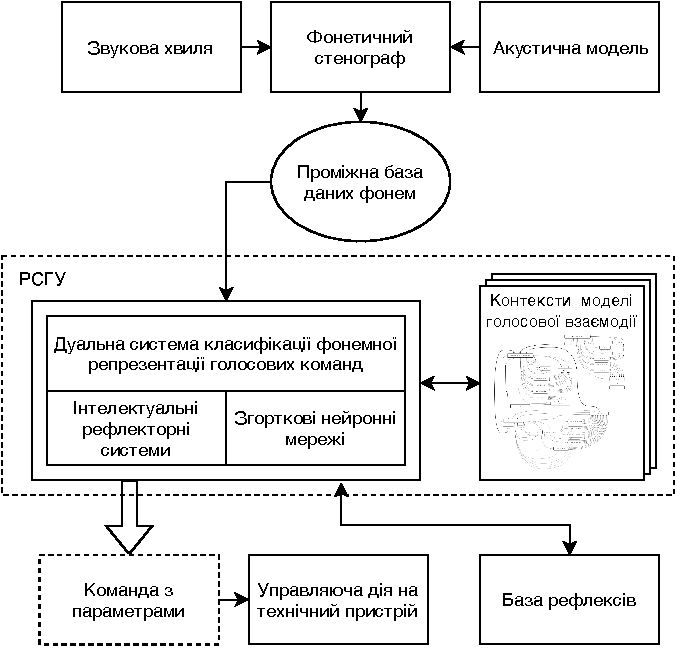
\includegraphics [width=.6\linewidth] {rsgu_struct_new}
	\caption{Удосконалена схема системи формалізації голосової інформації в моделі голосової взаємодії водія при диспетчерському контролі за рухом автотранспорту}
	\label{img:rsgu_struct_new}
\end{figure}

\FloatBlock

Метод інтелектуальних рефлекторних систем для класифікації голосових команд представлений у матричній формі полягає в наступному:

\begin{enumerate}
	\item Розрахунок визначеності для інтелектуальної системи відносно всіх вхідних N-грам фонем і можливих голосових команд:
	
	\begin{align}
		D_A&=\pm0.5(P_{A}\oslash(J_{1,p}-P_{A}) + (J_{1,p}-P_{A})\oslash P_{A} -2J_{1,p})^{\circ \frac{1}{2}}; \nonumber \\
		D_{AB}&=\pm0.5(P_{AB}\oslash(J_{p,q}-P_{AB}) + (J_{p,q}-P_{AB})\oslash P_{AB}-2J_{p,q})^{\circ \frac{1}{2}}; \nonumber \\
		I_A&=(D_A^{\circ 2}+J_{1,p})^{\circ \frac{1}{2}};\quad I_{AB}=(D_{AB}^{\circ 2}+J_{p,q})^{\circ \frac{1}{2}}, \nonumber
	\end{align}
	
	де: $p=|A|$ --- потужність множини голосових команд;
	
	{\settowidth{\leftskip}{де:\ }
	
		$q=|B|=\sum_{i=s_{\text{min}}}^{s_{\text{max}}}f^i$ --- потужність множини N-грам фонем,
		
		$f$ --- кількість фонем в акустичній моделі,
		
		$s_{\text{min}}$ та $s_{\text{max}}$ --- мінімальний та максимальний розміри N-грам;
		
		$J_{i,j}$ --- матриця одиниць розміром $i\times j$
		
		$P_{A}$ --- матриця безумовної ймовірності вибору команд з множини $A$ (розмір матриці $1\times p$); 
		
		$D_A$ --- матриця визначеності щодо команд з множини $A$; 
		
		$I_A$ --- матриця інформованості щодо команд з множини $A$; 
		
		$P_{AB}$ --- матриця умовної ймовірності вибору команд з множини $A$ при наявності впливу N-граму фонем з множини $B$ (розмір матриці $p\times q$); 
		
		$D_{AB}$ --- матриця визначеності щодо команд з множини $A$ при наявності впливу N-граму фонем з множини $B$; 
		
		$I_{AB}$ --- матриця інформованості щодо команд з множини $A$ при наявності впливу N-граму фонем з множини $B$
		
		$\circ$, ${}^{\circ}$ та $\oslash$ --- операції матричного поелементного добутку, піднесення до степеня та ділення Адамара.
		
	}
	
	\item Отримання додаткової визначеності, що є у N-грамів фонем відносно голосових команд:
	
	\[
	D_\Delta=D_{AB} \circ (J_{p,1}I_A)-I_{AB} \circ (J_{p,1}D_A),
	\]
	
	де $D_\Delta$ --- матриця додаткової визначеності щодо команд з множини $A$ яку надає наявність N-граму фонем з множини $B$ (розмір матриці $p\times q$).
	
	\item Розрахунок сумарного впливу на голосову команду, реакцію інтелектуальної системи всіх наявних N-грамів фонем:
	
	\[
	D_\Sigma = XD_\Delta;\quad I_\Sigma=(D_\Sigma^{\circ 2}+J_{n,q})^{\circ \frac{1}{2}},
	\]
	
	де: $n$ --- кількість вхідних команд для розпізнання або навчання системи; 
	
	{\settowidth{\leftskip}{де:\ }
		
		$X$ --- вхідна матриця команд для розпізнання або навчання системи представлений у форматі «мішок N-грам фонем», тобто матриці розміром $n \times p$, де $x_{ij}=1$ якщо для відповідної голосової команди $i$ існує N-грам фонем $j$, в інакшому випадку $x_{ij}=0$;
	
		$D_\Sigma$ --- матриця сумарної додаткової визначеності щодо команд  з множини $A$ під впливом всіх N-грамів фонем з множини $B$ (розмір матриці $n\times q$);
		
		$I_\Sigma$ --- матриця сумарної додаткової інформованості щодо команд  з множини $A$ під впливом всіх N-грамів фонем з множини $B$.
		
	}
	
	\item Обчислення нової інформованості та визначеності голосової команди:
	
	\[
	D_Y=D_\Sigma \circ (J_{n,1}I_A) - I_\Sigma \circ (J_{n,1}D_A);\quad I_Y=(D_Y^{\circ 2}+J_{n,q})^{\circ \frac{1}{2}},
	\]
	
	де $D_Y$ --- матриця нової (вихідної) визначеності щодо команд  з множини $A$ під впливом всіх N-грамів фонем з множини $B$ (розмір матриці $n\times q$); 
	
	$I_Y$ --- матриця нової (вихідної) щодо команд з множини $A$ під впливом всіх N-грамів фонем з множини $B$.
	
	\item Обчислення сумісної умовної ймовірності команди $A_i$ (при наявності всіх N-грамів фонем $B_j \in B$):
	
	\[
	Y=P_Y=0.5J_{n,p}+D_Y \oslash 2I_Y,
	\]
	
	де $P_Y$ --- матриця сумісної умовної ймовірності команд з множини $A$ під впливом всіх N-грамів фонем з множини $B$.
\end{enumerate}

Як альтернативний класифікатор фонетичного тексту голосової команди запропоновано метод згорткових нейронних мереж, що широко використовується в різноманітних задачах класифікації звукових даних та природно-мовних текстів. Цей метод полягає в наступному:

\begin{enumerate}
	\item Представлення кожної фонеми у вигляді one-hot вектору;
	\item Розрахунок одновимірного згорткового шару з фільтрами розмірами 2, 3 та 4 і кроком 1;
	\item Розрахунок агрегаційного шару виділенням максимального значення кожного фільтру;
	\item Конкатенація результатів обрахунку всіх фільтрів;
	\item Розрахунок повнозвʼязного шару з функцією активації ReLU та нормалізацією Dropout;
	\item Розрахунок точності та функції втрат.
\end{enumerate}

Таким чином система формалізації голосової інформації в моделі голосової взаємодії водія при диспетчерському контролі за рухом автотранспорту містить фонемний стенограф та згорткову нейронну мережу, яка працює з фонемами. Реалізація ЗНМ виконана на мові Python з використанням TensorFlow. Нейронна мережа містить паралельні одновимірні шари з різними варіантами кроку фільтра з активаційною неспадаючою диференційованою функцією ReLU; фонеми представляються у вигляді one-hot вектору, фрази нормалізовані за максимальною довжиною, з використанням вектора з усіма нулями в якості заповнювача. Для навчання використано Adam-алгоритм зворотного розповсюдження помилки із стохастичним градієнтним спуском, який дозволяє регулювати величину швидкості навчання в залежності від параметрів. Для зниження ефекту перенавчання ЗНМ використано Dropout шар. Також побудовано алгоритм зворотного поширення помилки ЗНМ. 

Метод інтелектуальних рефлекторних систем представлено у термінах нейронних мереж, шо дає можливість отримати оптимальні значення параметрів рефлекторних систем $p(A_i/B_j)$ та $p(A_i)$ не традиційним частотним методом обрахунку, а шляхом навчання методом зворотного розповсюдження помилки.

У \textbf{четвертому розділі} «Засоби формалізації голосової інформації в системах диспетчерського контролю за рухом автотранспорту» описано розроблені засоби формалізації голосової інформації в системах диспетчерського контролю за рухом автотранспорту, особливості їх використання, проведене експериментальне дослідження ефективності засобів та впровадження.

На основі запропонованих методів та моделей розроблено засоби формалізації голосової інформації, які дозволяють водію не відволікатись від управління автомобілем і слідкувати за дорожніми умовами та обстановкою, що дає змогу прискорити доставку продукції в процесі дистрибуції, а також підвищити рівень безпеки.

Розглянуті особливості використання розроблених засобів формалізації голосової інформації в системах диспетчерського контролю за рухом автотранспорту показали, що водію автомобіля, який буде здійснювати доставку продукції в процесі дистрибуції і вперше зіштовхнеться із засобом формалізації голосової інформації, що діє в рамках системи диспетчерського контролю за рухом автотранспорту, необхідно попередньо перевірити і при потребі донавчити систему розпізнавати його голосові команди з відповідних контекстів.

Процес порівняння ефективності різних методів класифікації в дуальній моделі формалізації голосової взаємодії експериментально перевірено за допомогою моделювання розпізнавання команд на основі ітеративного процесу збору даних та введення нових критеріїв оцінки, якщо попередні не дали достатньої точності оцінювання.
Використано розширений набір метрик оцінки ефективності моделей класифікації, що включав крім оцінки точності ще робастні метрики для незбалансованої вибірки (прецизійність, повноту, F-міру) та візуальний аналіз матриць помилок.

Оцінку ефективності дуальної системи формалізації голосової інформації проведено експериментальним шляхом у три етапи: на першому етапі первинного моделювання виявлено необхідність збільшення кількості вхідних даних; на другому перевірено гіпотезу недостатності кількості вхідних даних; на третьому --- гіпотезу недостатньої якості звукового сигналу. Прийнятний для практичного використання рівень точності в моделі, побудованій методом згорткових нейронних мереж досягнуто на другому етапі моделювання, а в моделі, побудованій методом інтелектуальних рефлекторних систем --- на третьому.

Результати третього етапу моделювання обома описаними методами наведені у таблиці \ref{tbl:data_total}. Розміри N-грам при моделюванні інтелектуальними рефлекторними системами були вибрані в діапазоні 2--4. Розміри згорткових фільтрів при моделюванні згортковими нейронними мережами також були взяті в діапазоні 2--4.

\begin{table}[!h]%
	\caption{Порівняння двох методів формалізації ІРС і ЗНМ}%
	\label{tbl:data_total}% label всегда желательно идти после caption
	%	\renewcommand{\arraystretch}{1.4}%% Увеличение расстояния между рядами, для улучшения восприятия.
	\def\tabularxcolumn#1{m{#1}}
	\begin{tabularx}{\textwidth}{@{}>{\centering}X | >{\centering}X >{\centering}X | >{\centering}X >{\centering}X | >{\centering}X >{\centering\arraybackslash}X@{}}% Вертикальные полосы не используются принципиально, как и лишние горизонтальные (допускается по ГОСТ 2.105 пункт 4.4.5) % @{} позволяет прижиматься к краям
		\toprule     %%% верхняя линейка
		№ Контексту & Точність ІРС & F-міра ІРС & Точність ЗНМ & F-міра ЗНМ & Кількість стимулів & Кількість реакцій \\
		\midrule %%% тонкий разделитель. Отделяет названия столбцов. Обязателен по ГОСТ 2.105 пункт 4.4.5 
		1 & 0.850 & 0.590 & 0.900 & 0.900 & 100 & 2 \\
		3 & 0.866 & 0.862 & 0.997 & 0.997 & 350 & 7 \\
		4 & 0.870 & 0.867 & 0.990 & 0.990 & 200 & 4 \\
		5 & 0.830 & 0.830 & 0.967 & 0.966 & 300 & 6 \\
		6 & 0.835 & 0.829 & 0.975 & 0.975 & 200 & 4 \\
		7 & 0.774 & 0.775 & 0.948 & 0.948 & 500 & 10 \\
		8 & 0.857 & 0.851 & 0.983 & 0.983 & 300 & 6 \\
		9 & 0.884 & 0.737 & 0.976 & 0.976 & 250 & 5 \\
		10 & 0.864 & 0.865 & 0.960 & 0.960 & 250 & 5 \\
		11 & 0.824 & 0.814 & 0.952 & 0.951 & 250 & 5 \\
		12 & 0.751 & 0.753 & 0.951 & 0.950 & 450 & 9 \\
		13 & 0.813 & 0.620 & 0.927 & 0.926 & 150 & 3 \\
		14 & 0.730 & 0.734 & 0.950 & 0.950 & 300 & 6 \\
		15 & 0.780 & 0.778 & 0.923 & 0.922 & 300 & 6 \\
		16 & 0.840 & 0.832 & 0.968 & 0.968 & 250 & 5 \\
		17 & 0.646 & 0.641 & 0.951 & 0.952 & 350 & 7 \\
		18 & 0.740 & 0.739 & 0.928 & 0.928 & 250 & 5 \\
		19 & 0.825 & 0.821 & 0.980 & 0.980 & 200 & 4 \\
		По всій вибірці & 0.637 & 0.628 & 0.890 & 0.890 & 3200 & 64 \\
		\bottomrule %%% нижняя линейка
	\end{tabularx}%
\end{table}

Впровадження протягом року у трьох дистрибуційних компаніях підтвердило ефективність розробленої інформаційної технології формалізації голосової інформації: система підтримки диспетчеризації автотранспорту підвищує загальну ефективність процесу доставки за рахунок скорочення кількості необхідних транспортних засобів та підвищення кількості точок які можуть бути обслуговуванні одним транспортним засобом; запровадження голосового інтерфейсу може підвищити відсоток уникнення чи виправлення водіями інцидентів і відхилень від планового маршруту.

Для апробації розроблених засобів, систему підтримки диспетчеризації автотранспорту було впроваджено на підприємстві ТОВ «Українські Інформаційні Технології» та досліджено її використання протягом року у трьох підприємствах-клієнтах.

Результати цієї апробації показали загальне підвищення ефективності процесу доставки на 14.5\%, за рахунок скорочення кількості необхідних транспортних засобів на 7.1\% та підвищення кількості точок які можуть бути обслуговуванні одним транспортним засобом в середньому на 9.4\%.

%\FloatBlock

При цьому дослідження показали, що в залежності від навантаженості доби, від 5\% до 15\% точок доставки повʼязані з певними інцидентами та відхиленнями від плану, і лише 10\% з цих інцидентів вдається ліквідувати або надолужити. Статистичне моделювання проведене на основі порівняння поведінки різних водіїв показало, що водії які вчасно повідомляють про можливі інциденти через додаток з сенсорним управлінням можуть уникнути чи виправити до 50\% інцидентів, а отже запровадження голосового інтерфейсу може розповсюдити ці результати на всіх водіїв.

\section*{Висновки}

%% Согласно ГОСТ Р 7.0.11-2011:
%% 5.3.3 В заключении диссертации излагают итоги выполненного исследования, рекомендации, перспективы дальнейшей разработки темы.
%% 9.2.3 В заключении автореферата диссертации излагают итоги данного исследования, рекомендации и перспективы дальнейшей разработки темы.
У дисертаційній роботі вирішено актуальне наукове завдання розробки моделей і методів формалізації голосової інформації в системах диспетчерського контролю за рухом автотранспорту. Загалом можна зробити наступні висновки.

1. Дослідження теоретико-методологічних засад формалізації голосової інформації в системах дистрибуції показало, що значну роль в їх управлінні відіграють процеси голосової взаємодії особливо стосовно своєчасного коригування планових маршрутів руху автотранспорту. Розроблення моделі голосової взаємодії без блоку переведення звуку голосу в текст може принципово покращити автоматизацію голосової взаємодії в системах контролю дистрибуції.

%Сучасний етап автоматизації голосового управління в організаційно-технічних системах характеризується проблемою вчасного корегування маршруту, що призводить до витрат часу на комунікацію. Встановлено, що процес автоматизації управління в системах дистрибуції повинен включати етап моніторингу руху автомобілів у режимі реального часу, а існуючі системи є занадто простими, що не зможуть справитись з задачами дистрибуції для використання в управлінні транспортними доставками.

2. Розроблена система автоматичного розрахунку планових маршрутів та практика її використання забезпечили накопичення параметрів непередбачуваних ситуацій в процесі доставки, що впливають на створення сценаріїв голосової взаємодії, які представляються у вигляді орієнтованого графу та контекстів взаємодії. 
Принципи побудови рефлекторних систем на основі теорії несилової взаємодії адаптовано для формалізації голосової інформації в системах диспетчерського контролю за рухом автотранспорту.

%Проаналізовані сучасні інформаційні системи обробки та формалізації голосової інформації показали існування достатньої кількості таких методів. Встановлено, що недоліком традиційних систем розпізнання мови є те, що вони не забезпечують автоматизацію голосової взаємодії в задачах управління дистрибуцією, оскільки це потребує додаткових технічних та телекомунікаційних засобів. Орієнтуючись на новітні підходи до автоматизації голосової взаємодії встановлено необхідність застосування теорії несилової взаємодії з рефлекторною системою голосового управління, що включає аналіз інформаційної складової та виконання відомої реакції відповідним обʼєктом.

3. Розроблено модель голосової взаємодії субʼєктів дистрибуції в системах диспетчерського контролю за рухом автотранспорту, яка представлена у вигляді повного графу сценаріїв усіх етапів дистрибуції «склад – дорога – точка доставки». Виділено перелік унікальних контекстів голосової взаємодії, формалізація голосової інформації в яких може відбуватися незалежно, що дозволяє знизити кількість реакцій для автоматизованого розпізнання.

%Під час дослідження процесу автоматизації руху автотранспорту в дистрибуції та розгляд принципів побудови рефлекторної системи голосової взаємодії встановлено, що найбільш перспективним напрямом, який дає змогу запропонувати нове принципове рішення і побудувати рефлекторну модель голосової взаємодії в задачах управління дистрибуцією є застосування моделей логічних сценаріїв взаємодії у процесах дистрибуції, які мають враховувати параметри основних причин невідповідності реальної ситуації запланованому маршруту. Тому набула подальшого розвитку модель на трьох етапах дистрибуції, проблемні моменти в якій вирішуються із залученням диспетчера для вибору найкращої стратегії і мінімізації втрат, яка є основою для побудови дерева сценаріїв голосової взаємодії для кожного з субʼєктів (диспетчера та водія). Дерево сценаріїв запропоновано будувати у вигляді орієнтовного графу і використовувати такі сутності як: Контекст або Стан, Стимул або Подія, Реакція системи відповідно до стимулу. Крім того, для побудови рефлекторної системи голосової взаємодії встановлено закономірності застосування теорії несилової взаємодії як основи інтелектуальних рефлекторних систем та теоретично запропоновано використовувати рефлекторний метод в системі голосової взаємодії диспетчерського контролю за рухом автотранспорту.

4. Створено метод формалізації голосової інформації в системах підтримки диспетчеризації автотранспорту з використанням інтелектуальних рефлекторних систем, що дозволяє автоматизувати голосову взаємодію субʼєктів дистрибуції з уникненням переводу звукової інформації в лексичний текст за рахунок використання двох основних модулів (автоматичного фонетичного стенографа і ядра рефлекторної системи голосового управління). Для реалізації ядерного компонента запропоновано дуальну систему класифікації голосових команд, яка може використовувати метод інтелектуальних рефлекторних систем або метод згорткових нейронних мереж.

%Під час розгляду методів формалізації голосової інформації в системах диспетчерського контролю за рухом автотранспорту вперше отримано модель голосової взаємодії водія в системах диспетчерського контролю за рухом автотранспорту, яка представлена у вигляді дерева сценаріїв усіх етапів дистрибуції «склад – дорога – точка доставки» та визначено перелік контекстів та можливих реакцій на них.

%В системі формалізації голосової інформації в моделі голосової взаємодії водія при диспетчерському контролі за рухом автотранспорту удосконалено процес формалізації голосової інформації, що складається з двох основних модулів: автоматичного фонетичного стенографа і ядра рефлекторної системи голосового управління, поточна реалізація яких визначає умови їх використання в моделі голосової взаємодії;

%Для формалізації голосової інформації вперше запропоновано використовувати згорткові нейронні мережі. У даному випадку система формалізації голосової інформації в моделі голосової взаємодії водія при диспетчерському контролі за рухом автотранспорту містить фонемний стенограф та згорткову нейронну мережу, яка працює з фонемами.

%Крім того, отримали подальший розвиток інтелектуальні рефлекторні системи, що призначені для формалізації голосової інформації, що представлені у термінах згорткових нейронних мереж та, які дають можливість отримати оптимальні значення параметрів шляхом навчання методом зворотного розповсюдження помилки.

5. Оцінка ефективності дуальної системи формалізації голосової інформації проведена експериментальним шляхом у три етапи: на першому етапі первинного моделювання виявлено необхідність збільшення кількості вхідних даних; на другому перевірено гіпотезу недостатності кількості вхідних даних; на третьому --- гіпотезу недостатньої якості звукового сигналу. Прийнятний для практичного використання рівень точності в моделі, побудованій методом згорткових нейронних мереж досягнуто на другому етапі моделювання, а в моделі, побудованій методом інтелектуальних рефлекторних систем --- на третьому.

Аналіз результатів моделювання показав що застосування дерева сценаріїв та розбиття повного набору команд на контексти є доцільним, оскільки значення точності без використання контекстів є найменшими для обох методів класифікації. Порівняння результатів моделювання для різних методів класифікації показало що обидва методи можуть бути використані на практиці, причому навчання моделі при використанні методу інтелектуальних рефлекторних систем набагато швидше ніж для згорткових нейронних мереж, але фактичне розпізнавання на навченій системі відбувається швидше з використанням згорткових нейронних мереж. Точність моделювання також вища при використанні згорткових нейронних мереж.

6. Впровадження протягом року у трьох дистрибуційних компаніях підтвердило ефективність розробленої інформаційної технології формалізації голосової інформації: система підтримки диспетчеризації автотранспорту підвищує загальну ефективність процесу доставки за рахунок скорочення кількості необхідних транспортних засобів та підвищення кількості точок які можуть бути обслуговуванні одним транспортним засобом; запровадження голосового інтерфейсу може підвищити відсоток уникнення чи виправлення водіями інцидентів і відхилень від планового маршруту.

%У результаті проведених експериментальних досліджень формалізації голосової інформації, отриманої від водіїв, набув подальшого розвитку процес моделювання рефлекторними системами, в якому отримано нові дані під час апробації засобів формалізації голосової інформації в системах диспетчерського контролю за рухом автотранспорту, які призначені для оптимізації диспетчерського контролю за рухом автотранспорту при виконанні процесів дистрибуції. Крім того, результати досліджень при апробації засобів формалізації голосової інформації в системах диспетчерського контролю за рухом автотранспорту показали те, що з підвищенням загальної кількості стимулів відбувається зріст розпізнаних стимулів, що призводить до збільшення точності розпізнання.



\ifdefmacro{\microtypesetup}{\microtypesetup{protrusion=false}}{} % не рекомендуется применять пакет микротипографики к автоматически генерируемому списку литературы
\ifnumequal{\value{bibliosel}}{0}{% Встроенная реализация с загрузкой файла через движок bibtex8
  \renewcommand{\bibname}{\large \authorbibtitle}
  \nocite{*}
  \insertbiblioauthor           % Подключаем Bib-базы
  %\insertbiblioother   % !!! bibtex не умеет работать с несколькими библиографиями !!!
}{% Реализация пакетом biblatex через движок biber
  \ifnumgreater{\value{usefootcite}}{0}{
%  \nocite{*} % Невидимая цитата всех работ, позволит вывести все работы автора
  \insertbiblioauthorcited      % Вывод процитированных в автореферате работ автора
  }{
  \insertbiblioauthor           % Вывод всех работ автора
%  \insertbiblioauthorgrouped    % Вывод всех работ автора, сгруппированных по источникам
%  \insertbiblioauthorimportant  % Вывод наиболее значимых работ автора (определяется в файле characteristic во второй section)
  \insertbiblioother            % Вывод списка литературы, на которую ссылались в тексте автореферата
  }
}
\ifdefmacro{\microtypesetup}{\microtypesetup{protrusion=true}}{}

\section*{Анотація}

\textbf{\thesisAuthorLastName~\thesisAuthorInitials\ \thesisTitle.} --- Кваліфікаційна наукова праця на
правах рукопису.

Дисертація на здобуття наукового ступеня \thesisDegree\ за
спеціальністю \thesisSpecialtyNumber\ – «\thesisSpecialtyTitle». --- \thesisOrganizationDone, \thesisCity, \thesisYear.

Дисертаційна робота присвячена вирішенню актуальної науково-практичної задачі --- розробці моделей і методів формалізації голосової інформації в системах диспетчерського контролю за рухом автотранспорту. Розроблено інформаційну технологію: модель голосової взаємодії субʼєктів дистрибуції (яка представлена у вигляді повного графу сценаріїв усіх етапів дистрибуції «склад – дорога – точка доставки»); метод формалізації голосової інформації в системах підтримки диспетчеризації автотранспорту з використанням інтелектуальних рефлекторних систем; дуальна система класифікації голосових команд (яка налаштована на предметну область і використовує метод інтелектуальних рефлекторних систем або метод згорткових нейронних мереж у залежності від того, який з них ефективніший); засоби формалізації голосової інформації у вигляді мобільного додатку для системи Android. Використання експериментально перевіреної інформаційної технології здатне підвищити ефективність управління процесом дистрибуції.

\textbf{Ключові слова}: \keywords.

\section*{Аннотация}

\textbf{Найдёнов И. М. Информационная технология формализации голосовой информации в системах диспетчерского контроля за движением автотранспорта.} --- Квалификационний научный труд на правах рукописи.

Диссертация на соискание ученой степени кандидата технических наук по специальности 05.13.06 -- «информационные технологии». --- Киевский национальный университет имени Тараса Шевченко, Киев, 2018.

Диссертация посвящена решению актуальной научно-практической задачи --- разработке моделей и методов формализации голосовой информации в системах диспетчерского контроля за движением автотранспорта. Разработана информационная технология: модель голосового взаимодействия субъектов дистрибуции (которая представлена в виде полного графа сценариев всех этапов дистрибуции «склав -- дорога -- точка доставки»); метод формализации голосовой информации в системах поддержки диспетчеризации автотранспорта с использованием интеллектуальных рефлекторных систем; дуальная система классификации голосовых команд (которая настроена на предметную область и использует метод интеллектуальных рефлекторных систем или метод сверточных нейронных сетей в зависимости от того, какой из них эффективнее); средства формализации голосовой информации в виде мобильного приложения для системы Android. Использование экспериментально проверенной информационной технологии способно повысить эффективность управления процессом дистрибуции.

\textbf{Ключевые слова}: интеллектуальные рефлекторные системы; сверточные нейронные
сети; голосовое взаимодействие; распознавание речи; фонетический текст; системы дистрибуции; маршруты доставки; последняя миля.

\section*{Annotation}

\textbf{Naydonov I. M. Information technology of the formalization of voice information in systems of dispatch control of vehicle traffic.} --- Manuscript.

Thesis for the degree of candidate of technical sciences in the specialty 05.13.06 -- «information technologies». --- Taras Shevchenko National University of Kyiv, Kyiv, 2018.

Thesis research is devoted to the solution of the scientific and practical problem --- the development of models and methods for the formalization of voice information in dispatch control systems of vehicle traffic. The information technology of the formalization of voice information in dispatch control systems of vehicle traffic was developed: the model of voice interaction of distribution entities in dispatch control systems of vehicle traffic (which is presented as a complete communication script graph of all stages of the distribution «depot - road - delivery point»); the method of formalizing the voice information in vehicle dispatching support systems using intelligent reflex systems; dual system of classification of voice commands (which is tuned to the subject area and uses the method of intelligent reflex systems or the method of convolutional neural networks, depending on which of them is more effective); tool for formalizing voice information as a mobile application for the Android system. The use of experimentally proven information technology can improve the management of the distribution process.

%Дисертаційна робота присвячена вирішенню актуальної наукової задачі − розробці моделей і методів формалізації голосової інформації в системах диспетчерського контролю за рухом автотранспорту. Була розроблена інформаційна технологія формалізації голосової інформації в системах диспетчерського контролю за рухом автотранспорту: модель голосової взаємодії субʼєктів дистрибуції в системах диспетчерського контролю за рухом автотранспорту (яка представлена у вигляді повного графу сценаріїв усіх етапів дистрибуції «склад – дорога – точка доставки»); метод формалізації голосової інформації в системах підтримки диспетчеризації автотранспорту з використанням інтелектуальних рефлекторних систем; дуальна система класифікації голосових команд (яка налаштована на предметну область і використовує метод інтелектуальних рефлекторних систем або метод згорткових нейронних мереж у залежності від того, який з них ефективніший); засоби формалізації голосової інформації у вигляді мобільного додатку для системи Android. Використання експериментально перевіреної інформаційної технології здатне підвищити ефективність управління процесом дистрибуції.

The scientific novelty of the obtained results is that the scientific problem of integration of models and methods of formalization of voice information with the management of the distribution process has been solved for the first time in a single system of voice information formalization in dispatch control systems of vehicle traffic. Herewith, a model of voice interaction of distribution entities in dispatch control systems of vehicle traffic was developed for the first time, which is presented as a complete communication script graph of all stages of the distribution «depot - road - delivery point», which allows to narrow the scope of voice interaction to the boundaries of the subject area; a method for formalizing voice information in vehicle dispatching support systems using intelligent reflex systems was created for the first time, which allows automating voice interactions; the method of convolutional neural networks was further developed for the classification of voice commands in order to formalize the voice information in the systems of dispatch control of vehicle traffic, which was applied to phonemic text; the methods of constructing of intelligent reflex systems was further developed based on the use of neural networks to formalize the interaction processes, which makes it possible to obtain optimal values of the parameters of the reflex systems by trainig using the backpropagation method.

%Наукова новизна отриманих результатів полягає в тому, що вперше вирішено наукову проблему інтеграції моделей і методів формалізації голосової інформації з управлінням процесом дистрибуції в єдиній системі формалізації голосової інформації в системах диспетчерського контролю за рухом автотранспорту. При цьому вперше розроблено модель голосової взаємодії субʼєктів дистрибуції в системах диспетчерського контролю за рухом автотранспорту, яка представлена у вигляді повного графу сценаріїв усіх етапів дистрибуції «склад – дорога – точка доставки», що дозволяє звузити сферу голосової взаємодії до меж предметної області; вперше створено метод формалізації голосової інформації в системах підтримки диспетчеризації автотранспорту з використанням інтелектуальних рефлекторних систем, що дозволяє автоматизувати голосову взаємодію; набув подальшого розвитку метод згорткових нейронних мереж для класифікації голосових команд з метою формалізації голосової інформації в системах диспетчерського контролю за рухом автотранспорту, що полягає в застосуванні до фонемного тексту; та отримали подальший розвиток методи побудови інтелектуальних рефлекторних систем на основі використання нейронних мереж для формалізації процесів взаємодії, шо дає можливість отримати оптимальні значення параметрів рефлекторних систем шляхом навчання методом зворотного розповсюдження помилки.

The developed system of automatic calculation of planned routes and the practice of its use ensured accumulation of parameters of unpredictable situations in the delivery process, which influence the creation of voice interaction scenarios, which are presented in the form of a targeted graph and interaction contexts.
The principles of constructing reflex systems based on the non-force interaction theory are adapted for the formalization of voice information in systems of dispatch control of vehicle traffic.

%Розроблена система автоматичного розрахунку планових маршрутів та практика її використання забезпечили накопичення параметрів непередбачуваних ситуацій в процесі доставки, що впливають на створення сценаріїв голосової взаємодії, які представляються у вигляді орієнтованого графу та контекстів взаємодії.
%Принципи побудови рефлекторних систем на основі теорії несилової взаємодії адаптовано для формалізації голосової інформації в системах диспетчерського контролю за рухом автотранспорту.

The evaluation of the effectiveness of the dual system for the formalization of voice information was conducted experimentally in three stages: on the first stage of the primary modeling, the need to increase the number of input data was identified; on the second stage, the hypothesis of insufficient number of input data is checked; on the third --- the hypothesis of insufficient quality of the sound signal. Acceptable for practical use, the level of accuracy in the model built by the method of convolutional neural networks is achieved at the second stage of modeling, and in the model, built by the method of intelligent reflex systems --- on the third.

%Оцінка ефективності дуальної системи формалізації голосової інформації проведена експериментальним шляхом у три етапи: на першому етапі первинного моделювання виявлено необхідність збільшення кількості вхідних даних; на другому перевірено гіпотезу недостатності кількості вхідних даних; на третьому --- гіпотезу недостатньої якості звукового сигналу. Прийнятний для практичного використання рівень точності в моделі, побудованій методом згорткових нейронних мереж досягнуто на другому етапі моделювання, а в моделі, побудованій методом інтелектуальних рефлекторних систем --- на третьому.

Analysis of modeling results showed that the use of script graph and splitting a full set of commands to several contexts are appropriate, since the value of accuracy without contexts are the lowest for both methods of classification. Comparing the simulation results for different classification methods showed that both methods can be used in practice, and learning models using intelligent reflex systems much faster than convolution neural networks, but the actual recognition is faster using convolution neural networks. The accuracy of simulation is also higher using convolution neural networks.

%Аналіз результатів моделювання показав що застосування дерева сценаріїв та розбиття повного набору команд на контексти є доцільним, оскільки значення точності без використання контекстів є найменшими для обох методів класифікації. Порівняння результатів моделювання для різних методів класифікації показало що обидва методи можуть бути використані на практиці, причому навчання моделі при використанні методу інтелектуальних рефлекторних систем набагато швидше ніж для згорткових нейронних мереж, але фактичне розпізнавання на навченій системі відбувається швидше з використанням згорткових нейронних мереж. Точність моделювання також вища при використанні згорткових нейронних мереж.

The developed tool for formalizing voice information in the form of a mobile application for the Android system allows the driver to not distract from driving and monitor road conditions that can accelerate the delivery of products during the distribution, as well as increase the level of security.

%Розроблений засіб формалізації голосової інформації у вигляді мобільного додатку для системи Android дозволяє водію не відволікатись від управління автомобілем і слідкувати за дорожніми умовами та обстановкою, що дає змогу прискорити доставку продукції в процесі дистрибуції, а також підвищити рівень безпеки.

Actual implementation during the year in three distribution companies confirmed the effectiveness of the developed information technology for the formalization of voice information: vehicle dispatching support system increases the overall efficiency of the delivery process by reducing the number of vehicles needed and increasing the number of points that can be serviced by one vehicle; the introduction of a voice interface can increase the percentage of avoiding or correcting incidents and deviations from the planned route by drivers.

%Впровадження протягом року у трьох дистрибуційних компаніях підтвердило ефективність розробленої інформаційної технології формалізації голосової інформації: система підтримки диспетчеризації автотранспорту підвищує загальну ефективність процесу доставки за рахунок скорочення кількості необхідних транспортних засобів та підвищення кількості точок які можуть бути обслуговуванні одним транспортним засобом; запровадження голосового інтерфейсу може підвищити відсоток уникнення чи виправлення водіями інцидентів і відхилень від планового маршруту.

\textbf{Keywords}: intelligent reflex systems; convolution neural network; voice interaction; speech recognition; phonetic text; distribution system; delivery routes; last mile

%\newpage
%\section*{Для нотаток}
